\section{Results}

The main design goal of PIX is to produce efficient instrumented code. 
To invetigate the efficiency of instrumented executables by PIX, we ran several experiments 
on a selection of benchmarks from the the SPECCPU2000
Integer benchmark suite. All of the experiments are run on a
one core of a quad-core 2.4GHz IA32 Intel Xeon running Red Hat linux Enterprise 4.1.2 (linux kernel 2.6.18).

The first set of experiments quantifies the overhead of the program reorganization for instrumentation 
described in section \ref{Subsection:Relocation}. The instrumentation used is a simple basic block counter to count
the execution count of each basic block in an application run. Recall that this technique adds an additional unconditional
branch to each function call in order to relocate the function, extends all of the branches in the code
to use 32-bit offsets, and pads each basic block whose size is fewer than 5 bytes with nops so that a
5 byte jump can be inserted. We performed these transformations on our benchmark set then ran the resulting executable
to see the performance effects of our function relocation method on the unaltered executable. 

Figure \ref{Figure:RelocOverhead} presents
the runtime overhead seen in the modified executable as a percentage of the original application runtime.
The figure shows that the maximum slowdown due to function relocation modifications is 6.5\%, with an
average slowdown of just 1.6\% with respect to the original execution times. Of the popular dynamic instrumentation toolkits 
we have discussed so far (Pin, DynamoRIO, Valgrind and Dyninst), the lowest overhead for performing no instrumentation
on a x86 platform is average of 38\% when using DynamoRIO, where the highest overhead is 113\% on the same benchmark
set \cite{luk2005pin}. This shows that the relocation method that PIX uses has a minimal
performance impact on the performance of the applications and thus is a suitable approach for use as a basis for
producing efficient instrumented code.

\begin{figure}[ht]
\centering
\label{Figure:RelocOverhead}
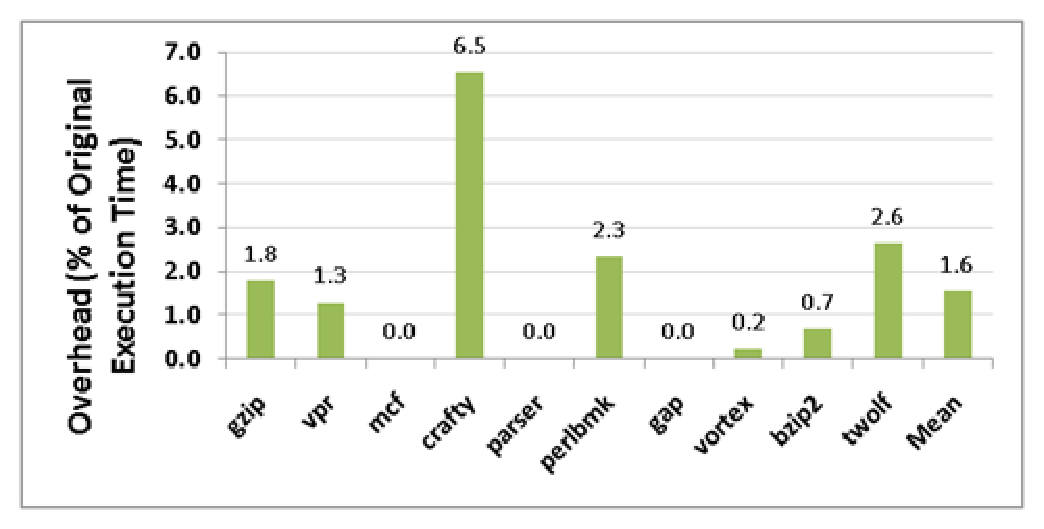
\includegraphics[scale=0.6]{relocperf.eps}
\caption{Application slowdown caused by preparing the code for instrumentation but without
any instrumentation inserted.}
\end{figure}

The next set of experiments shows how much overhead is introduced due to counting the
basic block executions in the code. We use this particular instrumentation tool because basic block counting
is a typical example of an instrumentation tool where we would expect PIX to generate efficient instrumented executables
as the number of instrumentation required is high. Much of the work performed in basic block counting (updating a single
counter every time a basic block is encountered) can be done easily using a fast instrumentation snippet rather than
by a full instrumentation function. These counters embodied in the instrumentation snippets must also be
persistent throughout the entire run of the application, which is more suited to a static instrumentation approach
because the static instrumentation does not utilize any resources to determine whether instrumentation can be removed.
The basic block counting instrumentation tool is used to produce an instrumented
executable for each program in our benchmark suite, whose runtime is compared to the runtime of the 
unmodified original executable. The results of these experiments are shown in figure \ref{Figure:ToolOverheads}. 

The figure \ref{Figure:ToolOverheads}
presents the overhead introduced as a percentage of the original application runtime. The
resulting overhead of our basic block counter ranges from XX-YY\% for the applications we tested with an average of 
84\% compared to their original executions More importantly, the figure shows that the overhead instroduced by PIX instrumentation is significantly 
lower compared to other instrumentation toolkits. The average overhead is 135\% for Pin (ranges between X-Y\%), 
396\% for DynamoRIO(ranges between X-Y\%), 660\% for Valgrind(ranges between X-Y\%), and XXX\% for Dyninst(ranges between X-Y\%). 
Our experiments demostrate that instrumented executable by PIX runs
51\% faster in the average compared to the next most efficient instrumentation toolkit, Pin. Furthermore,
Pin uses a variety of optimizations such as tracking eflags bit liveness \cite{luk2005pin} that are currently
unincorporated into PIX. We plan to incorporate more optimizations to PIX in the future (see Section \ref{Section:Future}) including
the optimizations already in use by Pin, which should further improve the efficiency of the instrumented
executables generated by our tool. 


\begin{figure}[ht]
\centering
\label{Figure:ToolOverheads}
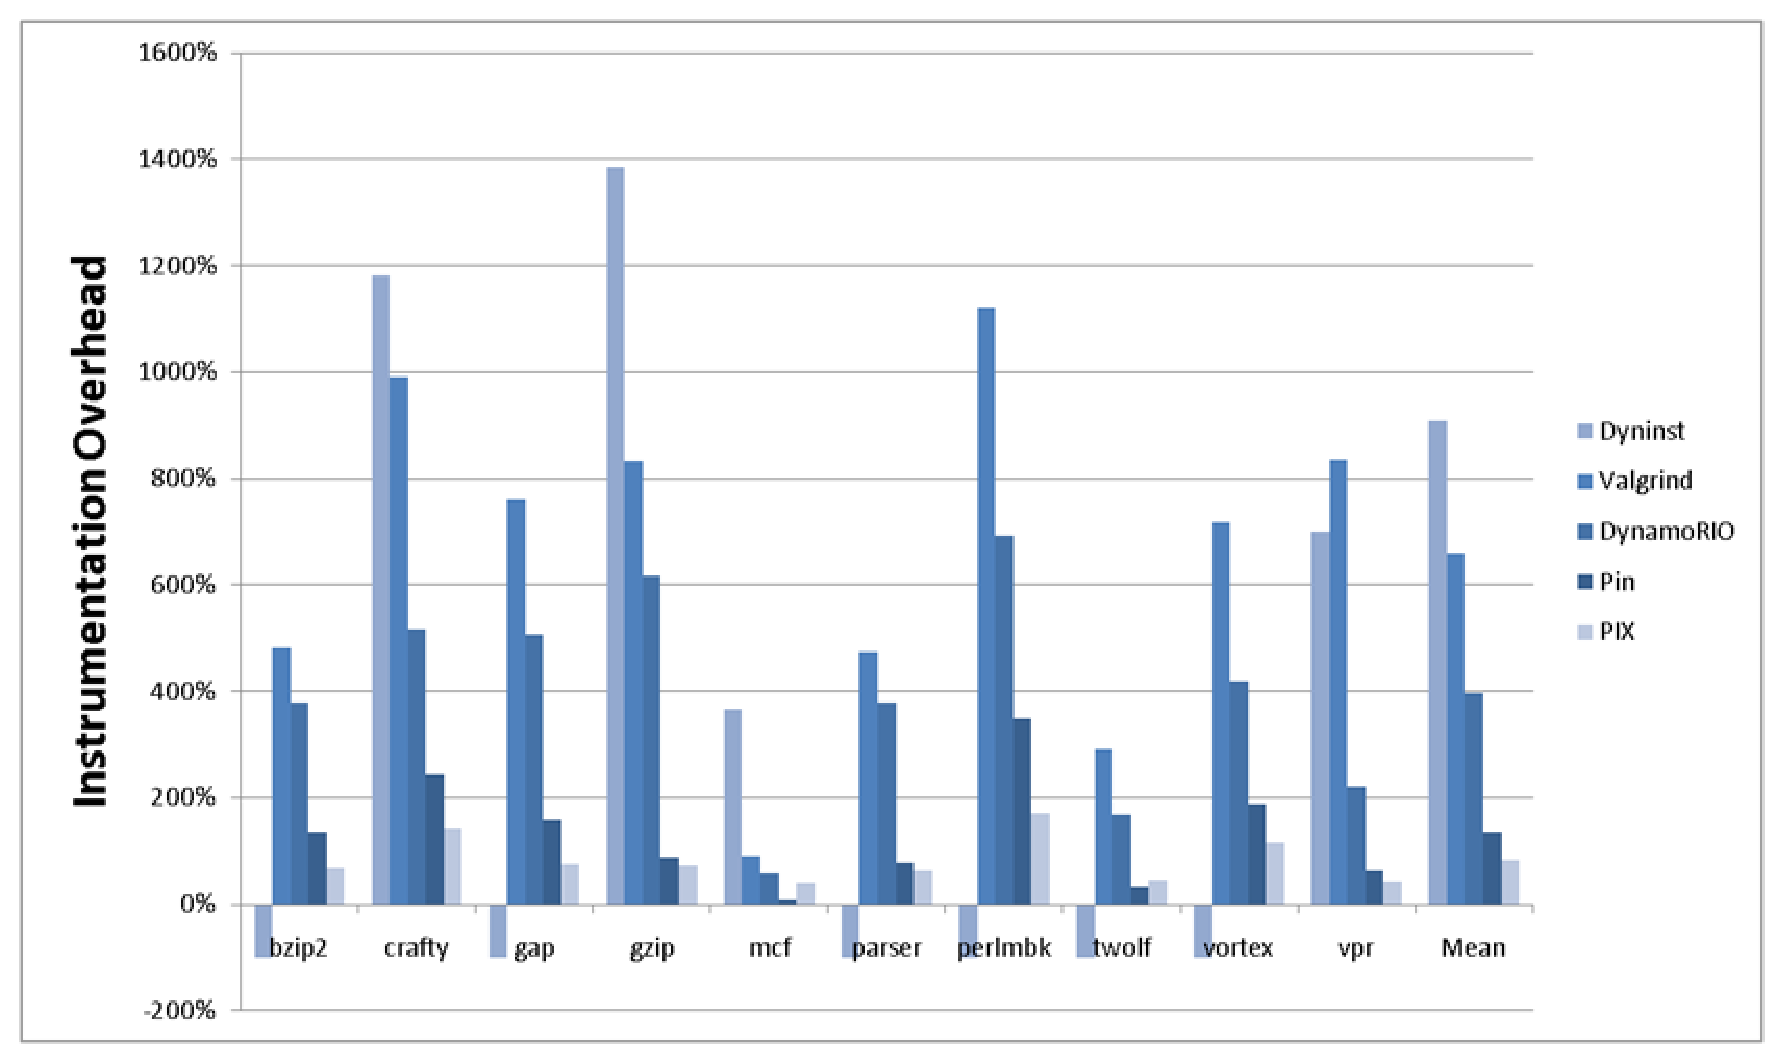
\includegraphics[scale=0.5]{bbcount.eps}
\caption{Performance of several x86 instrumentation tools with basic block counting instrumentation.}
\end{figure}

Overall Figures \ref{Figure:RelocOverhead} and \ref{Figure:ToolOverheads} demostrate that PIX instrumentation 
toolkit generates efficient instrumented executables and
outperforms other instrumentation toolkits for SPECCPU2000 Integer suite. We expect PIX to outperform even more in 
existence of high amount of instrumentation required by the instrumentation task such as memory address stream collection
where each load and store instruction is instrumented.